\chapter{Mean Shift Algorithm Analysis} % (fold)
\label{cha:algorithm_analysis}
Before any porting can be started the developer has to find out if there are 
multiple activities or tasks which can run simultaenously to expose exploitable 
concurrency. The developer has to find concurrency either by decomposing the  
data or tasks. By this decomposition one wants to solve bigger problems in less 
time as several processing units can solve different parts of the problem. 

But before any analysis is started one has to know if the problem is large enough
and if the resulting speedup justifies all the effort that is expended on making
a parallel version out of it. In case of mean shift which is used for several 
things like filtering, segmentation, pattern recognition and real time tracking
one can deduce that for bigger images or many images the computation time climbs
fast as the size or the number of images rises. To have a clue how the mean 
shift algorithm behaves with big pictures several run times where recorded.
For the analysis of the mean shift algorithm a ready to use \gls{EDISON} 
was used that was profiled and modified and parallelized for the purpose of this 
thesis.

The
\gls{EDISON}\footnote{http://www.caip.rutgers.edu/riul/research/code/EDISON/index.html}
system which was developed by the authors  \citeauthor{citeulike:462300} of
\citep{citeulike:462300} offers functionality to filter, segment and detect
edges in images. 

The \autoref{fig:cpu_run_time}
shows results of \gls{CPU} run times of the \gls{EDISON} application dependant
on image size. The vertical axis shows the run time in seconds and the
horizontal axis shows the side length in pixels of the quadratic \autoref{fig:orig0}.

\begin{figure}[ht]
\centering
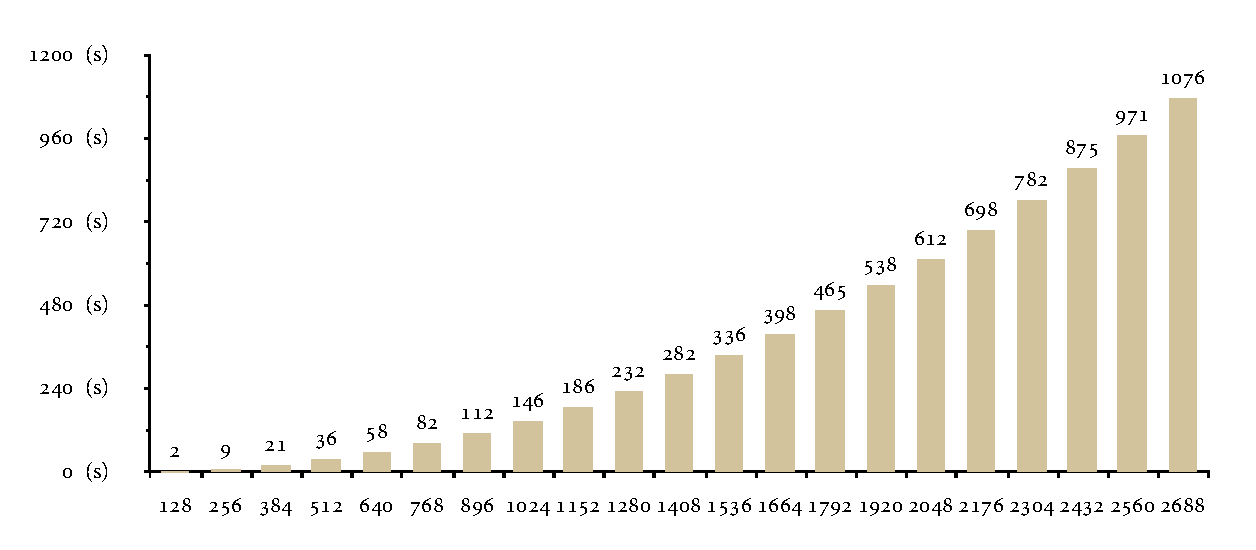
\includegraphics[width=390pt]{gfx/cpu_run_time}
\caption{CPU run time depending on the image size}
\label{fig:cpu_run_time}
\end{figure}

Considering the numbers in the result one can see that the run times grow 
linear to the image sizes. The mean shift algorithm has linear complexity, 
hence its complexity can be written as $O(n)$. Doubling the side length of 
the quadratic picture the run time increase by a factor of 4. See e.g.
the run times for side length: (l=256, t=9) and (l=512, t=36). 

But this is obviuos, as stated in \autoref{ch:mean_shift} for each pixel of the
image the mean shift vector has to be calculated, and if one increases the number
of pixels by a number $n$ we have to deal with $n$ times longer run time. Such 
consideration have to be done in the run-up to have a clue to which point the 
algorithm can be accelerated. The problem has to be well understood. 

The next important step is to find parts which can be offloaded to an accelerator
as the \gls{GPU}. A first good point for such parts is to make a profiling of 
the application to find out the most computationally intensive parts. It makes no
sense to parallelize functions which contribute only 1\% to the run time. 

\section{Profiling the Original Code} % (fold)
\label{sec:run_time_analysis_of_the_original_code}
A good start point is to take a profiler und generate a profile of the
functions, recording their run time and call history. In this case a statistical
profiler is used which operates by sampling. The samples are taken from the
hardware performance counters which every modern \gls{CPU} has builtin.
OProfile\footnote{http://oprofile.sourceforge.net/news/} a system wide profiler
for Linux was used to examine the run time of the \gls{EDISON} program. The
\autoref{tab:comp} shows the run time analysis of \gls{EDISON}.

\begin{table}[ht]
   \myfloatalign
	\rowcolors{2}{gray!10}{}
  \begin{tabularx}{\textwidth}{cclcc} \toprule
    \tableheadline{Self} & 
	\tableheadline{Total} & 
	\tableheadline{Symbol} &
	\tableheadline{Size} &
	\tableheadline{Module}\\ \midrule
	0,0\% &	100,0\% &	main &											589B & edison \\  
	0,0\% & 	100,0\% & 	Run(CmCParser*) &								576B & 	edison \\ 
	0,0\% & 	100,0\% & 	EXECUTE(int, CmCParser*, void**) &				1,24KB &	edison \\ 
	0,0\% & 	100,0\% & 	EDISON::Segment() &								27B & 	edison \\
	0,0\% & 	100,0\% & 	EDISON::meanShift(int) &							2,75KB & edison \\ 
	0,0\% & 	99,3\% &    msImageProcessor::Filter(...) &  676B & edison \\
	0,4\% & 	99,1\% & 	msImageProcessor::NonOptimizedFilter(...) &		1.007B & edison \\ 
	0,6\% & 	98,8\% & 	MeanShift::LatticeMSVector(double*, double*) &	250B & 	edison \\ 
	\color{Brown4}98,2\% & 	\color{Brown4}98,2\% & 	
	\color{Brown4}MeanShift::uniformLSearch(double*, double*) & 	\color{Brown4}1,01KB & \color{Brown4}edison \\ 
	0,0\% & 	0,4\% & 	msImageProcessor::FuseRegions(float, int) &		1,17KB & edison \\ 
	0,1\% & 	0,3\% & 	msImageProcessor::BuildRAM() &					2,29KB & edison \\ 
	0,0\% &	0,2\% & 	msImageProcessor::TransitiveClosure() &			1,63KB & edison \\
	0,0\% & 	0,2\% & 	msImageProcessor::Prune(int) &					1,56KB & edison \\ 
	0,0\% & 	0,2\% & 	msImageProcessor::GetResults(unsigned char*) & 	340B & 	edison \\
	0,1\% & 	0,2\% & 	msImageProcessor::LUVtoRGB(...) &				542B & 	edison \\
	0,2\% & 	0,2\% & 	RAList::Insert(RAList*) &						249B & 	edison \\
	0,0\% & 	0,1\% & 	msImageProcessor::DefineImage(...) &				356B & 	edison \\
	0,1\% & 	0,1\% & 	msImageProcessor::RGBtoLUV(...) &				556B & 	edison \\
	0,0\% & 	0,1\% & 	msImageProcessor::Connect() &					455B & 	edison \\
	0,1\% & 	0,1\% & 	msImageProcessor::Fill(int, int) & 				440B & 	edison \\
	0,1\% & 	0,1\% & 	msImageProcessor::InWindow(int, int) & 			372B &	edison \\
	0,0\% & 	0,0\% &	msImageProcessor::GetBoundaries() &				39B & 	edison \\
	0,0\% & 	0,0\% & 	msImageProcessor::SqDistance(int, int) & 			256B & 	edison \\ 
	0,0\% & 	0,0\% & 	msImageProcessor::DefineBoundaries() &			1,41KB & edison \\ 
    \bottomrule
  \end{tabularx}
  \caption[EDISON run time profile]{\gls{EDISON} run time analysis}
  \label{tab:comp}
\end{table}

Before taking a closer look at the table, the columns have to be explained. The
column {\textsc{total}} shows how long the function plus their child function
were executing. Whereas the column {\textsc{self}} shows how long the function spent
executing itself without the execution time of their child functions. The
column {\textsc{SYMBOL}} shows the function that was executed and the remaining
columns are irrelevant for now.

Now having a look at the table there is one function which is executing 98.2\%
of the run time, the function \emph{MeanShift::uniformLSearch(double*,
double*)}. In this function the algorithm tries to find feature points that fall
into the search window with radius $h$ (see \autoref{sec:mean_shift}). This is
the starting point as it is the most computationally intensive and the focus for
parallelization. There is a way to calculate to which extent the particular
function can be parallelized and which speedup one can expect. Speedup is the 
ratio of run time when executing a program on a single processr to the run time
when using $n$ processors. Given $T_1$ the run time of a program on a single
processeor and $T_n$ the run time of the same program on $n$ processors then
\begin{equation}\label{eq:speedup}
	S(n) = \frac{T_1}{T_n}
\end{equation}
is a measure for the speedup. One familiar law to calculate the how much speedup
can be obtained through paralellism is Amdahl's law. 

\section{Amdahl's law} 
\label{sec:amdahl_s_law}
Amdahl's law says supposing that 80\% of a computation can be parallelized and
20\% can't, then even if the 80\% that is parallel were run on an infinite
number of processors the highest speedup that one can achieve is 5. Generally
speaking if a fraction $p$ of a computation can be run in parallel and the rest
must run serially, Amdahl's law upper bounds the speedup by $1/(1-p)$.

The speedup of a application according to Amdahl is given by
\begin{equation}\label{eq:amdahl} 
	S_{max}(n) = \frac{1}{(1-p) + \frac{p}{n}}
\end{equation} 
where $1$ is the execution unit time of the old computation, $(1-p)$ the
inherently serial part and $p/n$ the parallel part divided by $n$ the
number of processing units. When $n \rightarrow \infty$ then the execution time
approaches the time for executing the sequential program fraction. So no matter
how many processors one adds to the system it will at least execute as long as
the sequential program fraction, which is an upper bound of speedup. A important
addition is that the sequential program fraction or serial processing percentage
is relative to the overall execution time using a single processor. It is 
independent of the number $n$ of processors \citeauthor{citeulike:3838998} 
\citep{citeulike:3838998}. 


Assuming that the mean shift filtering can be parallelized with any number of
processing units one can calculate the maximum speedup achieveable according
to Amdahl. Taking the parallel processing percentage from \autoref{tab:comp} for 
the filtering step: 
\begin{equation*}\label{eq:parallel}
	p = 99,3\% = 0.993 
\end{equation*}
we get

\begin{equation*}\label{eq:am0}
	S_{max}(n) = \frac{1}{(1-0.993)} = \frac{1}{0.007} = 142.857	
\end{equation*}

Applying the calculation with $n = 128$, the used \gls{GPU} has 128 processors one
can acheive a speedup of:
\begin{equation*}\label{eq:g92sp}
		S_{max}(128) = \frac{1}{(1-0.993) + \frac{0.993}{128}} = \frac{1}{0.007 + 0.0077578125} = 67.76
\end{equation*}

One can see that even for very small serial processing percentage the speedup is
not very high. Therefore \citeauthor{citeulike:3732921} proposed a alternative
formulation where the fractions are now dependent on $n$. He assumed that for 
larger problem, the fraction of a program to parallelization increases. Thats
why Gustafson's law is often referred as a scaled speedup measure
and Amdahl's as a non scaled speedup measure. Given the serial $s'$ and paralllel 
time $p'$ a single processor would require $s' + p' \times n$ time to finish the execution.
The speedup is then given by:
\begin{equation}\label{eq:gus}
	S_{max}(n) = \frac{s' + p' * n}{s' + p'} = n + ( 1 - n ) * s'
\end{equation}

Applying the calculation with $n = 128$, the used \gls{GPU} has 128 processors one
can acheive a speedup according to Gustafson of:
\begin{equation*}\label{eq:g92sp}
		S_{max}(128) = 128 + (1 - 128) * 0.007 = 127.11
\end{equation*}


It looks like that Amdahl's \& Gustafson's law are in contradiction but looking
more precise on both definitions one can see that both laws employ different
definitions for the fraction of the serial and parallel exectuion times. Amdahl
uses non scaled percentage and Gustafson scaled percentage. Mathematicaly they
are equal just two different formulations. The scaled percentage can be
transformed to a non scaled perecentage where Gustafson's law gives the same
results as Amdahl's law \citep{citeulike:3838998}.

In summary one can expect more than a 100 fold speedup when parallelizing the
filter step of the mean shift algorithm. The next steps will  focus on analyzing
how the mean shift filter can be decomposed to take advantage of 
multiple processors.

\section{Data and Task Parallelism} % (fold)
\label{sec:data_and_task_parallelism}


\subsection{Task Parallelism} % (fold)
\label{sub:task_parallelism}

There are two ways to decompose an algorithm to take advantage of parallelism.
The first way is to decompose the algorithm into several tasks that can run
independently. Each task is performing indepently different calculation on the
data. This characteristic is known as task parallelism. To know if two task can
run independent one can take \citeauthor{citeulike:6113408} conditions and
evaluate them.

Let $P_i$ and $P_j$ be two tasks of a program $P$. For $P_i$ let $I_i$ be the
input and $O_i$ the output data and for $P_j$ let $I_j$ be the input and $O_j$ 
be the output data, then $P_i$ and $P_j$ are independent if they satisfy the
following conditions \citep{citeulike:3838998}:  

\begin{subequations}\label{eq:bern_cond}
	\begin{align}
		I_j \cap O_i & = \emptyset \label{eq:bern0}\\ 
		I_i \cap O_j & = \emptyset \label{eq:bern1}\\
		O_i \cap O_j & = \emptyset \label{eq:bern2}
	\end{align}
\end{subequations}

Equipped with the knowledge how to identify independent parallel tasks, the 
mean shift segmentation algorithm \autoref{lst:segmalgo} can now be examined. 
Having a look at the algorithm steps one can easily see that every task is 
violating every condition stated above. The filtering step input data is 
dependent on the \gls{RGB} to \gls{LUV} conversion output data. The segmentation
step input data is dependent on the filtering output data and the output data 
of each step is written to the same location for each pixel. So it does not matter
how big an image is or if it is a color or grayscale image the mean shift segmentation
algorithm will always perform all from each other dependent calculations as
described in \autoref{lst:segmalgo}. The longest path of dependent calculations
is the critical path. For the mean shift algorithm there exist no shorter path. 

Having a look again at \autoref{tab:comp} where the most computationally 
intesive parts are identified, one could think of having different tasks for the
filtering step. But again here the same situation each calculation is inherently 
dependent on each other. 

In summary one can discard the idea of task parallelism for the mean shift
segmentation algorithm. Thats why the focus of parallelization is now on data
parallelism.
% subsection task_parallelism (end)


\subsection{Data Parallelism} % (fold)
\label{sub:data_parallelism}
The second way of decomposing an algorithm is data decomposition. The data is
decomposed into chunks on which similar operations are being applied in such a
way that the different chunks can be operated on concurrently. The focus in data
parallelism is on the data structures which define the problem and not at the
tasks.

Focusing on data and having a look at the most computational intensive part, 
the filtering step one can see that each pixel of an image can be calculated 
independently. The input and output pixels are independent and furthermore it
doesnt matter at which pixel one starts, the filtering step is deterministic, 
starting from the same input will lead to the same output. 

Another important aspect is how often the subtasks (where each subtask is
calculating one pixel) have to synchronize or communicate. An algorithm exhibits
fine-grained parallelism if the subtasks have to communicate many times,
coarse-grained parallelism if the subtasks do not communicate many times. In
this case the algorithm even exhibits embarrasingly parallel parallelism. The
subtasks never have to communicate or synchronize. Each subtask takes one or a
chunk of pixels applys the filtering steps and writes back the result. The
intermediate steps where the mean shift vector is moved over the spatial space
are also independent for each pixel.

The approach in parallelising the mean shift algorithm is to use a data
decomposition where each subtask is filtering a chunk of the image. Depending on
the number of processing units one can choose an apropriate chunk size to
exploit every unit.

If the algorithm would only exhibit fine-grained parallelism the next steps would
be to identify groups to simplify the job of managing dependencies and have a 
look at the ordering to satisfy contraints among tasks. Luckily here one has only
to deal with a embarrasingly parallel algorithm and can move to the next step, 
identify how data is accessed and shared among subtasks. 

\subsubsection{Data Flow} % (fold)
\label{ssub:data_flow}




% subsubsection data_flow (end)
 


% subsection data_parallelism (end)



% section data_and_task_parallelism




















